\chapter{Testing Environment}
\label{chap:testing_environment}
	
	\par In this chapter is described the whole environment where I settled the investigation of each Android mobile application discussed in this thesis.
	\par Core of the environment is the \textit{Android Studio} framework, offering both an Integrated Development Environment (IDE) and testing features for Android mobile applications. Here I configured an emulated device where I could run the application cases I investigated.
	\par Once installed the specific application I had to analyze the \textit{network traffic} generated by itself. Generally it is rare a single tool is perfect for all the applications to analyze, this is the reason why I used different tools to inspect the network traffic generated by an application, instead of just sticking with one tool. Starting from the standard-de-facto in packet inspection \textit{Wireshark} program, ending to tools acting like proxy servers between the client application and the server. Some of these tools are able to automatically install and configure a man (MitM attack [\ref{subsec:mitm}]) in the middle of the communication, others might need some manually configuration. \newline
	The whole amount of informations exchanged between application and server is hidden somewhere in the communication. It might be more or less difficult to find them, but all the informations are there, in those packets.
	\par Some tools revealed to be really useful while investigating the network traffic of the applications. Dynamic instrumentations tools are softwares able to inspect at runtime what is happening in the mobile application. On the other way, static instrumentation tools offer a view of the application basing on its code.
	
	\section{Android Studio}
		\par \textbf{Android Studio} is the center of the testing environment. Other than a complex IDE software, it provides a complete testing suite for Android mobile applications. Once installed the software, it enables the access to the Android Device Manager tool, where the user can create an emulator for a specific Android device choosing among phones, tablets, wearOS or TVs. 
		\par In this section I will explain how I prepared the android virtual device in order to obtain a working environment that made possible the application investigation.
		
		\subsection{Android Virtual Device (AVD)}
			\par For my purpose study case I created an \textit{Android Virtual Device} (AVD) phone with the same properties of the \textit{Pixel 3a} phone developed by Google, that is \textit{5.6''} screen size, \textit{1080x2220} resolution, \textit{440dpi} density. The device is running \textit{Android 13}, also known as \textit{Tiramisu} version, or \textit{API 33}, on \textit{x86\_64} architecture. In the really first step while selecting the hardware we would like to use for the virtual device, some device definitions are enabled to run the Play Store software, and so it is for our Pixel 3a device. This is really useful since I had not to download and install manually each applications on the device. Indeed it is made possible using the Google Play store directly from the emulated device. Here there is the full property list of the device I used:
			\begin{figure}[ht]    
				\centering   
				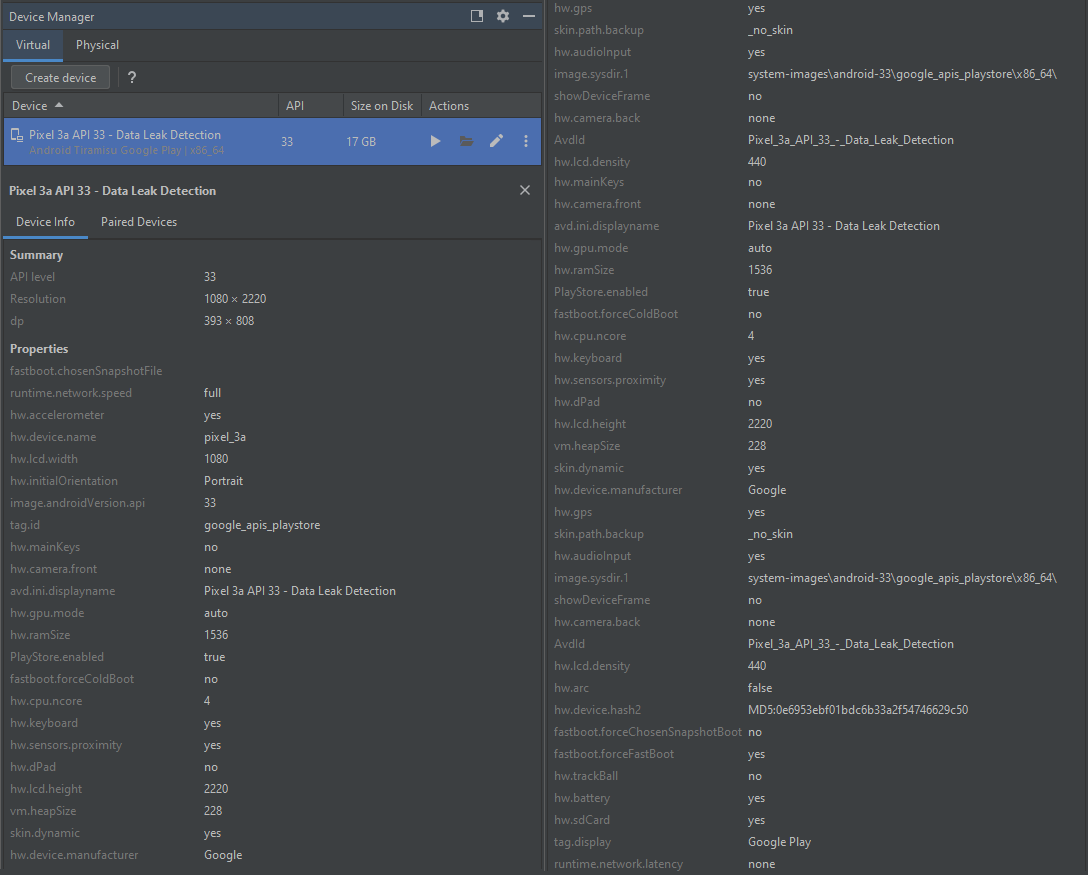
\includegraphics[width=0.9\textwidth]{./images/avd_splitted.png}
			    	\caption{Android Virtual Device (AVD) specifics}
			\end{figure}
			\par Once created the new virtual device (in my case called \textit{''Pixel\_3a\_API\_33\_-\_Data\_Leak\_Detection''}), it is possible to run it through the Android Device Manager. For simplicity I created a simple \textit{.bat} file to run the virtual device without the need to open Android Studio everytime. Indeed there is a file called \textit{emulator.exe} in a the folder where we installed the Android SDK. We can simply open the emulator by command line passing the name of our AVD and some optional arguments. Here it is how my command looks like:
\begin{lstlisting}[language=bash, caption={run\_AVD.bat}]
	C:\<Android_folder>\Sdk\emulator\emulator -feature -Vulkan -memory 2048 -netdelay none -netspeed full -avd Pixel_3a_API_33_-_Data_Leak_Detection
\end{lstlisting}
		\par More specifically the \textit{-feature -Vulkan} argument will force the emulator to do not use the \textit{Vulkan} graphic library. Since Android API 30 lots of android applications, such as Google Chrome, use this library to boost its performance. Anyway in some devices, especially for the emulated ones, might result in a massive slow rendering time. Other arguments are specifying to dedicate 2 Gb of RAM memory for the device, to not impose limits on the network speed and to not simulate any network delay.
			
		\subsection{Root privileges on virtual device}
			\par After having succesfully created the AVD, it can result useful to get the \textit{root privileges} on the device. In our case it is really mandatory since what we are going to do is intercept the communication protocol in the middle between application and server. As explained in the Section \ref{subsec:mitm}, the client application needs to trust the proxy server, and this is done by checking its certificate. Starting from the release of version \textit{Nougat} (API $\ge$ 24), of Android operative system, it changed the behaviour adopted by android applications in trusting users. If before the application was checking both \textit{user certificates} and \textit{system certificates}, now it will check exclusively the installed system level certificates, therefore root privileges are mandatory. \newline
			\par There are so many tools that let a user obtain the root privileges on his phone. I personally have used the \textit{rootAVD} tool available online \cite{rootAVD}. The procedure is really simple, firstly run the command with argument \textit{ListAllAVDs} to list all the AVDs on the machine. We will obtain the full path of our AVDs, that we will pass as argument when executing the tool from command line. The tool will make use the \textit{adb} tool that Android Studio brings together with its development tools, so it is worth it to explain what it is.
		
		\subsection{Android Debug Bridge (adb)}
			\par As I said Android Studio offers a complete set of features to run and test android application. In particular by installing the \textit{Android SDK Platform Tools} package from Android Studio, we will obtain a set of tools that make possible the debug of our application. \newline
			One of the most important tools is the Android Debug Bridge, more noticed as \textit{adb}. It is a command line tool that let the user directly communicate with an android device, let it be a real device or a physical one. Basically it is a client-server program that runs both on our machine and android device. There is then a client, that is the command line tool, a daemon \textit{adbd} running in the background of the android device, and a server managing the connection between client and daemon. For a complete understanding of the adb tool check the Android Developer guide \cite{adb}.
		
	\section{Network traffic analysis}
		\par Once the virtual device is well configured as described above, let's start introducing some tools used in the study case. Each one of them has some strengths, one tool might works for an application but not work for another. They are listed below in order of complexity. \textit{HttpToolkit} and \textit{BurpSuite} are network traffic interceptors, that means every connection outgoing from our device will be intercepted by these applications, letting the user to inspect more or less accurately how the request are formed. \textit{Wireshark} on the other way is a packet sniffing tool, meaning that it will capture any packet in the network, regardless of the protocol or port of them. 
		
		\subsection{HttpToolkit}
		\label{sec:http_toolkit}
			\par HttpToolkit\cite{http_toolkit} is an open-source tool for debugging, testing and building with HTTP(S). The strength of this tool relies on its simplicity for configuring the environment. Once downloaded the application it requires to connect to a source of traffic. In this case the network source to monitor is the android virtual device where the applications will run. HttpToolkit provides a variety of available sources, from the most famous browser (Chrome, Firefox, Safari, Edge), up to more complicated environment, such as Docker containers, virtual machines, Android devices or iOS devices. HttpToolkit itself will notify the user on which are the available sources of traffic at the start up. Since the scope of the study is investigating applications running on the android emulator, it is needed to download from Google Play the HttpToolkit application also on the virtual device. Once installed the android app, the HttpToolkit running on the computer will automatically notice the new source called \textit{''Android device via ADB''}. Just click on it and the whole proxy system is automatically configured. \newline
			\par In this phase it is crucial to understand what is happening:
			\begin{itemize}
				\item HttpToolkit is able to inject a custom certificate on our device, thanks to the ADB. Since we also have the root privileges on the android emulator, the certificate willl be placed in the folder of the \textit{System Certificates} that is \textit{/system/etc/security/cacerts} in the Android device. \newline
				\item The respective HttpToolkit android application will be activated in order to set up a VPN, redirecting the whole network traffic directly via the Android Debug Bridge. \newline
				\item HttpToolkit will copy to the device, again via ADB, a file containing the command used to start up the android Google Chrome application. This specific command will bypass the Certification Transparency check described in the section \ref{subsec:certification_transparency}. The command looks like the following:
\begin{lstlisting}
	chrome --ignore-certificate-errors-spki-list=<cert_digest>
\end{lstlisting}
			\end{itemize} 
			
			As described in the certificate verification [Section \ref{subsec:certificate_verification}] and MiTM [Section \ref{subsec:mitm}], this is the moment in which the HTTP(S) requests outgoing from the application case are intercepted by HttpToolkit, showing precisely each request detail. Then they are forwarded to the application server. Same happens for the HTTP(S) responses.
			\par This tool requires almost no configuration on the user side, all is done automatically aside from the preparation of the AVD discussed in the above section.
		
		\subsection{BurpSuite}
		\label{sec:burp_suite}
		
		\subsection{Wireshark}
		\label{sec:wireshark}
		
	
	\section{Dynamic instrumentation}
		\subsection{Frida}
		\subsection{Objection}
		
	\section{Static instrumentation}
		\subsection{GDA}
